\section{Incantations}
\label{sec:incantations}

The oldest spells are still the strongest~\cite{knuth}. A well-formed
incantation balances its braces and names its environment:
\begin{equation}
  \mathcal{P}(\text{compiles}) = \prod_{i=1}^{n} \left(1 - \varepsilon_i\right),
  \label{eq:success}
\end{equation}
where $\varepsilon_i$ is the chance that the $i$-th package disagrees with
the rest. Equation~\eqref{eq:success} explains why every new package is a
small act of faith.

\begin{figure}[h]
  \centering
  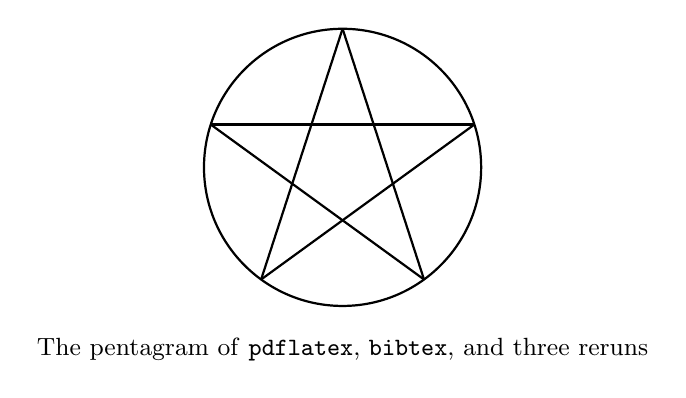
\begin{tikzpicture}[scale=1.1]
    \draw[thick] (0,0) circle (1.6);
    \foreach \a in {90,162,234,306,18}
      \draw[thick] (\a:1.6) -- ({\a+144}:1.6);
    \node at (0,-2.1) {\small The pentagram of \texttt{pdflatex}, \texttt{bibtex}, and three reruns};
  \end{tikzpicture}
  \caption{A standard summoning circle.}
  \label{fig:circle}
\end{figure}
